\documentclass[conference]{IEEEtran}
\IEEEoverridecommandlockouts

\usepackage[utf8]{inputenc}
\usepackage[T1]{fontenc}
\usepackage{lmodern}
\usepackage{graphicx}
\usepackage{amsmath,amssymb}
\usepackage{cite}
\usepackage{tikz}
\usetikzlibrary{arrows.meta,positioning}

\title{Educational Perspectives on Complementary FETs (CFET):\\
Evolution Beyond GAA and Open Challenges}

\author{
\IEEEauthorblockN{Shinichi Samizo}
\IEEEauthorblockA{Project Design Hub, Samizo-AITL\\
Email: samizo-aitl@example.com}
}

\begin{document}
\maketitle

\begin{abstract}
This tutorial paper provides an educational overview of emerging
\emph{Complementary FET (CFET)} technology, which vertically stacks
nFET and pFET devices beyond Gate-All-Around (GAA) nanosheets.
CFET reframes the CMOS inverter as a \emph{cross-sectional} integration,
promising density and delay improvements. We consolidate structure,
electrical impacts, fabrication challenges, and modeling limitations,
and articulate the pedagogical value of CFET as an open, unresolved
technology for semiconductor curricula.
\end{abstract}

\begin{IEEEkeywords}
CFET, GAA, FinFET, nanosheet FET, scaling, education, tutorial, vertical stacking, PDK.
\end{IEEEkeywords}

\section{Introduction}
Scaling has progressed from planar CMOS to FinFET and most recently
GAA nanosheet FETs. Beyond the 2\,nm node, interconnect delay and cell
area limit further gains. CFET (Complementary FET) stacks nFET and pFET
so that the cross-section itself forms a CMOS inverter, potentially
doubling effective cell density while shortening critical connections.
This paper positions CFET as both a roadmap element and an educational
vehicle for device--design co-optimization.

\section{Device Evolution}
Fig.~\ref{fig:evolution} sketches the historical trajectory.

\begin{figure}[t]
\centering
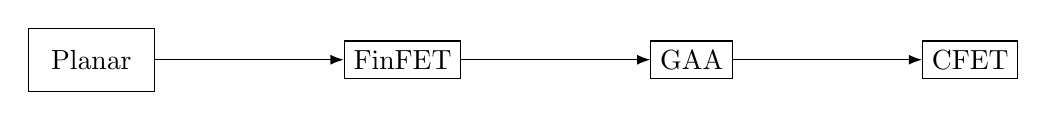
\begin{tikzpicture}[node distance=2.4cm,>=Latex]
\node[draw, minimum width=1.6cm, minimum height=0.8cm] (planar) {Planar};
\node[draw, right=of planar] (finfet) {FinFET};
\node[draw, right=of finfet] (gaa) {GAA};
\node[draw, right=of gaa] (cfet) {CFET};
\draw[->] (planar) -- (finfet);
\draw[->] (finfet) -- (gaa);
\draw[->] (gaa) -- (cfet);
\end{tikzpicture}
\caption{Device evolution: Planar $\rightarrow$ FinFET $\rightarrow$ GAA $\rightarrow$ CFET.}
\label{fig:evolution}
\end{figure}

\section{CFET Structural Concepts}
Two main variants are considered: (i) \emph{Sequential CFET}, where
the bottom device (e.g., nFET) is completed first and the top device
(e.g., pFET) is formed under a tight thermal budget; and (ii)
\emph{Forksheet CFET}, where n/p channels are arranged orthogonally to
alleviate routing congestion. Both integrate complementary devices in
the vertical dimension to realize \emph{cross-section = inverter}.

\begin{figure}[t]
\centering
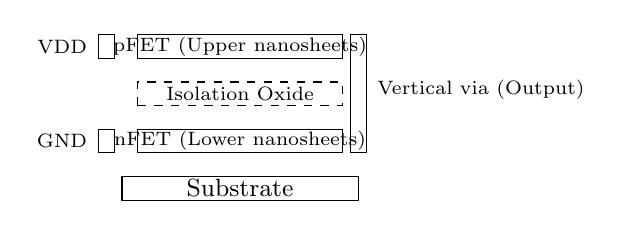
\begin{tikzpicture}[scale=1.0]
% Substrate
\draw (0,0) rectangle (3,0.3);
\node at (1.5,0.15) {\small Substrate};

% nFET
\draw (0.2,0.6) rectangle (2.8,0.9);
\node at (1.5,0.75) {\scriptsize nFET (Lower nanosheets)};

% Isolation oxide
\draw[dashed] (0.2,1.2) rectangle (2.8,1.5);
\node at (1.5,1.35) {\scriptsize Isolation Oxide};

% pFET
\draw (0.2,1.8) rectangle (2.8,2.1);
\node at (1.5,1.95) {\scriptsize pFET (Upper nanosheets)};

% Vias
\draw (2.9,0.6) rectangle (3.1,2.1);
\node[anchor=west] at (3.12,1.4) {\scriptsize Vertical via (Output)};
\draw (-0.3,0.6) rectangle (-0.1,0.9);
\node[anchor=east] at (-0.32,0.75) {\scriptsize GND};
\draw (-0.3,1.8) rectangle (-0.1,2.1);
\node[anchor=east] at (-0.32,1.95) {\scriptsize VDD};
\end{tikzpicture}
\caption{Sequential CFET cross-section: pFET stacked over nFET with vertical output via.}
\label{fig:cfet_stack}
\end{figure}

\begin{figure}[t]
\centering
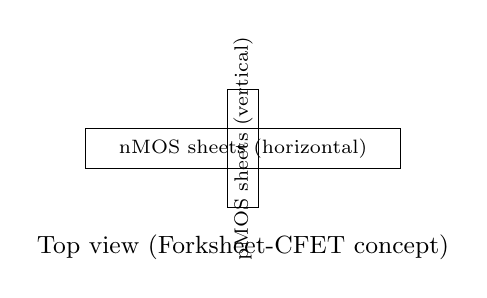
\begin{tikzpicture}[scale=1.0]
% Horizontal nMOS region
\draw (0,0) rectangle (4,0.5);
\node at (2,0.25) {\scriptsize nMOS sheets (horizontal)};
% Vertical pMOS region
\draw (1.8,-0.5) rectangle (2.2,1.0);
\node[rotate=90] at (2.0,0.25) {\scriptsize pMOS sheets (vertical)};
\node at (2,-1.0) {\small Top view (Forksheet-CFET concept)};
\end{tikzpicture}
\caption{Forksheet-CFET top view concept: orthogonal n/p nanosheets for routing relief.}
\label{fig:forksheet}
\end{figure}

\section{Electrical Features and Design Impacts}
Salient educational points include: (i) area efficiency approaching
$\sim\!2\times$ at the standard-cell level; (ii) reduced RC delay due
to vertical n/p connections; (iii) improved symmetry; and (iv)
emergent parasitics from vertical vias and inter-layer coupling.

\section{Manufacturing Challenges}
Key integration hurdles: independent n/p doping, thermal budget
separation, selective epitaxy/etching across multiple layers, and
BEOL co-design of VDD/GND and output vias with tight alignment.

\section{Modeling and EDA Limitations}
Compact models remain limited: BSIM-CMG covers GAA but not CFET;
Verilog-A prototypes exist without consensus; no CFET-ready PDKs or
standard-cell libraries are publicly available. This gap itself is
pedagogically valuable.

\section{Educational Value}
CFET links device physics with circuit/layout co-optimization and
exposes students to unresolved, multidisciplinary challenges---a
useful anchor for advanced semiconductor courses and capstone projects.

\section{Conclusion and Outlook}
CFET reframes CMOS as a stacked, cross-sectional inverter. While
pre-industrial, it motivates research in forksheet layouts, 3D-CFET,
and System-on-Stack integration. Embedding CFET in curricula helps
prepare engineers for the 2030s.

\section*{Acknowledgment}
The author thanks the Project Design Hub community for discussions.

\bibliographystyle{IEEEtran}
\bibliography{refs}

\end{document}
